\documentclass[12pt]{book}
\usepackage[utf8]{inputenc}
\usepackage[spanish]{babel}
%\usepackage{graphicx}
\usepackage[pdftex]{hyperref}
\usepackage{emp}
\usepackage{listings}
\usepackage{eurofont}

% Uncomment the following lines to put each section in a new page
%\usepackage{titlesec}
%\newcommand{\sectionbreak}{\clearpage}

%\usepackage{caption3} % load caption package kernel first
%\DeclareCaptionOption{parskip}[]{} % disable "parskip" caption option

\usepackage[font=scriptsize,format=plain,labelfont=bf,up,textfont=it,up]{caption}
%\usepackage[a4paper,margin=1cm,landscape]{geometry}
%\usepackage{tikz}
%\usetikzlibrary{positioning,shapes,shadows,arrows}

\ifx\pdftexversion\undefined
\usepackage[dvips]{graphicx}
\else
\usepackage[pdftex]{graphicx}
\DeclareGraphicsRule{*}{mps}{*}{}
\fi


\begin{document}
	
	\title{Programación mediante tarjetas gráficas\\Mejora de una aplicación distribuida}
	\author{Autor: Samuel Rodríguez Sevilla\\Tutor: José María Sierra Cámara}
	
	\maketitle
	
	\section*{}
	\pagebreak\newpage

	\vspace*{\fill}
	\begin{quote}
		Jesús le preguntó: <<¿Cuál es tu nombre?>>
		
		<<Legión>>, respondió, porque eran muchos los demonios que habían entrado en él.
		
		\emph{Lucas 8-30}
	\end{quote}
	\vspace*{\fill}
	
	\tableofcontents
	\listoffigures
	\listoftables
	
	\begin{empfile}
	\begin{empcmds}
	input metauml;
	\end{empcmds}
	% The rest of the document here
	\chapter{Introducción}

Uno de los puntos más débiles en la seguridad de toda organización ha sido las contraseñas. Cuando el usuario dispone de absoluto control sobre la decisión de cómo debe ser ésta, las contraseñas tienden a ser muy débiles ante ataques de diccionario. La solución a este problema reside en el uso de políticas de contraseña que exijan unos mínimos de fortaleza (uso de minúsculas y mayúsculas, números y símbolos). Estas políticas se pueden controlar informáticamente obligando al usuario poner contraseñas de calidad.

Por otra parte la potencia de las CPUs se ha incrementando, lo que ha supuesto la necesidad de mejorar los sistemas criptográficos para hacerlos más resistentes a todo tipo de ataques. En el caso concreto de las funciones resumen este fortalecimiento se ha materializado de dos formas distintas:

\begin{itemize}
	\item Se ha incrementado el número de bits del resumen para disminuir la posibilidad de colisiones.
	
	\item Se procura mejorar la técnica de generación del resumen para garantizar que los resúmenes sean lo más aleatorios posibles, utilizando procesos que impidan determinar el mensaje a partir del resumen y que garanticen estar normalmente\footnote{Si los resúmenes generados no tuviesen una distribución normal esto supondría que habría grupos de resúmenes y facilitaría ataques contra éstos pues sería más fácil determinar de dónde podrían proceder.} distribuidos. 
\end{itemize}

Estas mejoras ha ido esquivando uno de los problemas más importantes que han tenido las funciones resumen: el incremento de la potencia de las CPUs permite realizar ataques de fuerza bruta en tiempos asumibles.

El incremento de la potencia de las CPUs se ha visto restringido por la capacidad de integración de transistores en un microprocesador y el diseño interno del mismo. Si tomamos la Ley de Moore ésta dice que el número de transistores en un microprocesador tiende a duplicarse cada 18 meses. Esto nos permite planificar qué capacidad de cómputo podría tener un CPU en el futuro de cara a evitar ataques de fuerza bruta. De todos modos, el número de transistores es solo una parte de la capacidad de una CPU ya que su estructura interna afecta también de forma muy clara. Esto se debe a la forma que tiene de organizar la ejecución de una aplicación, la calidad del predictor de saltos, etc.

Al mismo tiempo a la mejora de las CPUs, se ha ido produciendo una importante mejora en las GPUs. Estos procesadores de propósito específico han visto su potencia incrementada muy rápidamente gracias a sus diseños más sencillos (se utilizan específicamente para cálculo matemático) y a su gran capacidad de paralelización (una NVIDIA Tesla puede disponer de hasta 970 núcleos) como puede verse en la Figura \ref{fig:GPUvsCPU}. Desde hace algún tiempo las tarjetas gráficas permiten cargar pequeños trozos de códigos denominados \emph{shaders} (éstos códigos se utilizan como filtros para efectos 3D) y esta técnica a desembocado en permitir la carga de códigos de usuario más genéricos.

\begin{figure}
	\centering
	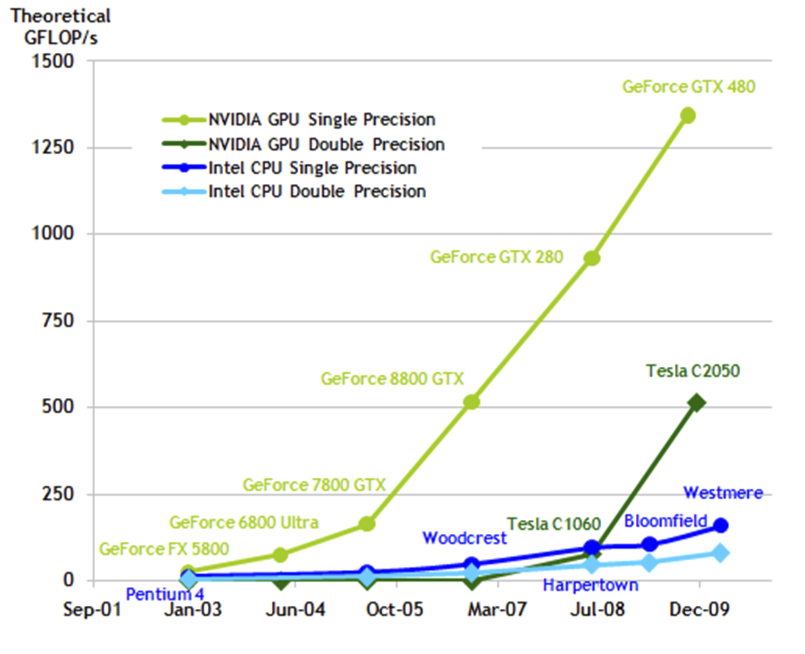
\includegraphics[width=0.7\textwidth]{evolucion-gpu.png}
	\caption{Comparativa de la evolución de los GFlops de las GPUs frente a las CPUs\cite{nvidia:cuda_c_programming_guide}}\label{fig:GPUvsCPU}
\end{figure}

La principal razón por la que el uso de GPU para computación se ha convertido en algo de interés es la publicación de APIs como CUDA y OpenCl que nos permiten aprovechar las capacidades de las actuales tarjetas gráficas para realizar cálculos y operaciones muy costosas en tiempo de CPU de forma más rápida. Además, permiten un alto grado de paralelismo, lo que puede resultar beneficioso para el desarrollo de ciertos tipos de programas.

En la actualizadad, mientras con una CPU se podía conseguir hasta 80 millones de claves MD5 por segundo (aplicando muchas optimizaciones a nivel de lenguaje ensamblador), una GPU potente puede alcanzar hasta cerca de los 2.000 millones de resúmenes por segundo. Esto es, una GPU es hasta 250 veces más rápida que la CPU para este tipo de cálculos, propiciado, principalmente, por su mayor capacidad de paralelización.

Si consideramos el hecho de que en la actualidad casi todos los nuevos equipos que se venden en el mercado disponen de aceleradoras gráficas y que es muy fácil crear una red de ordenadores zombis se debe considerar la mejora de los mecanismos de contraseña una prioridad por parte de las organizaciones. Por este motivo es importante disponer de herramientas que permitan comprobar la fortaleza de las contraseñas y evaluar la dificultad de realizar ataques a los distintos algoritmos de resumen existentes y en experimentación.

\section{Motivación}

Como ya se ha comentado, es importante garantizar la calidad de los algoritmos y contraseñas dentro de las organizaciones. Por este motivo nace este proyecto fin de carrera que pretende ser el inicio de una herramienta versátil, sencilla y atractiva que permita ofrecer a las distintas organizaciones un mecanismo para fortalecer su seguridad.

\section{Objetivos}

Para poder comprobar la fortaleza de una contraseña dada y para poder evaluar la resistencia frente a ataques de fuerza bruta de diferentes tipos de funciones resumen hace falta disponer de una herramienta adecuada. Para este fin existe una gran cantidad de herramientas, principalmente destinadas a la recuperación de contraseñas extraviadas, pero que su código es cerrado y su precio elevado. Aunque el precio puede no resultar un problema importante, consideramos que el uso de aplicaciones que no suministran su código fuente no es recomendable en el ámbito de la seguridad informática ya que es importante poder saber qué es lo que la herramienta hace y eso solo se puede determinar de forma fehaciente si ésta es de código abierto. Por otra parte, también es recomendable que la herramienta se software libre porque así, en caso de que el fabricante deje de dar soporte a la misma, tendríamos permiso para poder realizar modificaciones eliminando de este modo la dependencia con el vendedor.

El presente proyecto final de carrera nace con el objetivo de aprovechar las nuevas arquitecturas gráficas en el entorno de la auditoría de seguridad informática, especialmente en el ámbito de las funciones resumen. Igualmente se ha pretendido utilizar un modelo distribuido para mejorar la escalabilidad del sistema y así disponer de una herramienta potente que pueda ser ampliada según la necesidad del momento.

En concreto, se desea disponer de un sistema que:

\begin{itemize}
	\item Sea distribuido para aprovechar los recursos existentes en una red de ordenadores de forma sencilla.
	
	\item Permita ofrecer una alto grado de escalabilidad.
	
	\item Facilite su mantenimiento y mejora constante, con la posibilidad de añadir funcionalidades que inicialmente no estuvieran previstas desde el inicio.
	
	\item Se pueda administrar de forma sencilla.
\end{itemize}

\section{Estructura del documento}

Para facilitar la búsqueda a través del este documento, se provee de la siguiente guía de la organización interna del documento. Éste se divide en los siguiente capítulos:

\begin{description}
	\item[\ref{cap2}. Funciones resumen:] introducción a las funciones resumen y a los tipos de ataques que existen sobre ellas.
	\item[\ref{cap3}. Desarrollo con tarjetas gráficas:] se introduce la historia del desarrollo con tarjetas gráficas y a cómo se programa utilizando CUDA, el API de NVIDIA.
	\item[\ref{cap4}. Distributed Hash Cracker:] la chicha del PFC
	\item[\ref{cap5}. Conclusiones:]
	\item[\ref{cap6}. Trabajos futuros:]
\end{description}
	\chapter{Funciones resumen}\label{cap2}

Los sistemas destinados a ocultar o proteger información llevan usándose desde tiempos de la antigua Roma \cite{Luciano87cryptology:from} e incluso antes. Paralelamente se ha tratado siempre de crear las técnicas necesarias para poder acceder a dicha información sin ser el destinatario legítimo de la misma. Esto ha creado la necesidad de mejorar constantemente los mecanismos de cifrado para evitar que la información protegida no pueda ser utilizada salvo por aquellos a la que está destinada.

En la actualidad hay una gran cantidad de sistemas para la protección de información y se utilizarán unos u otros dependiendo de lo que se pretenda hacer. Concretamente existen 3 grandes grupos de mecanismos de seguridad:
\begin{itemize}
	\item Sistemas de cifrado de clave simétrica, que son aquellos que utilizan una clave para cifrar la información y esta clave debe ser conocida por todos aquellos que quieran tener acceso a información.
	\item Sistemas de cifrado de clave asimétrica, que utiliza dos juegos de claves, una pública y conocida por todo el mundo y otra privada que solo su propietario posee.
	\item Sistemas de un solo sentido o funciones resúmenes (también conocidas como funciones \emph{hash}).
\end{itemize}

Las funciones resumen, que son las que nos interesan para el presento proyecto fin de carrera, son aquellas que cumplen las siguientes características:

\begin{itemize}
	\item Son fáciles de calcular en un sentido, pero es muy complicado hallar su inversa y
	\item Que dada una entrada de longitud arbitraria siempre producirán una salida de longitud fija.
\end{itemize}

Este tipo de funciones son ampliamente utilizadas en el mundo de la seguridad como sistema para el almacenamiento de contraseñas de usuario, la generación de claves de sesión o la firma digital de documentos (por poner algunos ejemplos). Al ser ampliamente utilizadas es importante disponer de mecanismos para comprobar la fortaleza del mecanismo de funcionamiento como la fortaleza de la clave elegida.

A causa de su gran uso es necesario disponer de sistemas que comprueben la fortaleza de las contraseñas elegidas por los usuarios o de las claves de sesión que pueda generar un sistema de seguridad. El primer caso es importante para garantizar la seguridad de las organizaciones, impidiendo que los usuarios elijan contraseñas que puedan ser adivinadas o quebrantadas por posibles atacantes dando acceso a la información privada de ésta con los consiguientes problemas por posibles copias y/o borrados de información. El segundo caso es importante para garantizar que los sistemas seguros sean capaces de generar claves suficientemente robustas para impedir ataques externos.

\section{Comprobación de funciones resumen y contraseñas}

Existen dos formas básicas para comprobar la fortaleza de los mecanismos de seguridad. El primero es buscar debilidades en la propia función resumen que se va a utilizar. El segundo mecanismo es comprobar la calidad de la clave utilizada. Para este último caso lo más sencillo es utilizar un de mecanismo de fuerza bruta. Éste tipo de comprobación consisten en probar todas las combinaciones posibles entradas para generar resúmenes y éstos se cotejan con un resumen conocido previamente.

El mayor problema de los sistemas de fuerza bruta es que al tener que hacer muchas comprobaciones el tiempo que tardan en obtener una solución es muy elevado. Por este motivo es importante poder predecir el tiempo que dedicarán previamente para comprobar si vale o no la pena intentar realizar una comprobación de éste tipo.

Para poder calcular el tiempo que se necesitará para poder poder hacer una comprobación de fuerza bruta empezaremos por el caso genera. En éste, el tiempo máximo (el que recorre todas la combinaciones posibles) es de:

$$ T_{max}=t\sum^n_{i=m}k^i $$
 
Donde $m$ es la longitud mínima de la entrada, $n$ es la longitud máxima y $k$ es el número de símbolos posibles del alfabeto a utilizar. Finalmente $t$ representa el tiempo de cómputo de la función resumen.

Utilizando este sistema como referencia de peor caso es fácil medir las mejoras aportadas por otros algoritmos. De este modo, y tomando como referencia el trabajo realizado en este proyecto final de carrera, el simple uso de la paralelización utilizando un sistema de $C$ procesadores homogéneos nos proporciona unos tiempos de:

$$ T_{max}=t\sum^n_{i=m}\frac{k^i}{C} $$

En la actualidad, gracias a los avances en las comunicaciones y a los distintos procesadores es normal disponer de sistemas distribuidos heterogéneos. Éstos pueden contar con unas cuantas máquinas o cientos de miles. Para este tipo de casos es necesario disponer de una función general que tenga en cuenta la velocidad de cálculo en cada tipo de procesador en que vaya a ejecutarse la función resumen. Si disponemos de $p$ tipos de procesadores distintos y $C_j$ procesadores para cada tipo que tardan $t_j$ segundos en computar la función resumen ($1 \leq j \leq p$):

$$ T_{max}=\frac{\sum^n_{i=m}k^i}{\sum^p_{j=1}\frac{C_j}{t_j}}$$
 
Con esta información  se puede calcular cuál debe ser el tamaño del sistema a utilizar para poder comprobar la fortaleza de una contraseña en un tiempo determinado.

Por ejemplo, si dispusiéramos de un sistema que utilizara 2 tipos de procesadores diferentes para calcular una función resumen y que el primer procesador puede hacer una media de 25 millones de resúmenes por segundo y el segundo procesador puede hacer 1250 millones de resúmenes por segundo (éste caso se aproxima al uso de CPU+GPU). De cada procesador se dispone de 4 unidades. Además, nuestra clave está entre 6 y 8 caracteres de longitud y solo vamos a considerar letras minúsculas y números lo que supone 36 símbolos de entrada. Esto supone que el tiempo máximo que tardará el sistema en comprobar todas las combinaciones en las condiciones expuestas es de casi 9,5 horas.

Es fácil comprobar que utilizando sistemas de fuerza bruta para comprobar resúmenes se resuelve de forma lineal con respecto al número de procesadores.

A parte de los sistemas de fuerza bruta, existen muchas técnicas que han surgido a partir de la investigación de los distintos tipos de sistemas de resumen. Estos nuevos sistemas proceden de debilidades de los propios algoritmos y deben ser tenidos en cuenta a la hora de evaluar la fortaleza de las funciones resumen.

Aunque no es propósito del presente proyecto de fin de carrera implementar todos los sistemas de comprobación conocidos sí es importante tenerlos en cuenta para poder hacer comparaciones y valoraciones con respecto a las soluciones implementadas.

\subsection{Ataque de cumpleaños}

Este ataque a los sistemas de resúmenes consiste en que dado un mensaje $M$ cualquiera y una función resumen $H$, que genera resúmenes de longitud $L$ bits, se puede hallar un mensaje $M’$ probando combinaciones aleatorias en aproximadamente $1.2\sqrt{2^L}$ intentos \cite{website:wastahf} \cite{Oorschot:1994:PCS:191177.191231}(en caso de que la función resumen sea uniformemente distribuida).

El principio en el que se base este ataque se encuentra en un problema de teoría de la probabilidad conocido como problema del cumpleaños o paradoja del cumpleaños. Esta dice que un grupo de personas debe tener 23 individuos para que haya un 50\% de probabilidad de que dos cumplan hayan nacido el mismo día (figura \ref{fig:Birthday}).

El funcionamiento general es el siguiente:

$$
P(i, n) = \left\{
	\begin{array}{l l}
		1                        & \mbox{si $i = 1$}\\
		P(i-1, n)\frac{n-i+1}{n} & \mbox{si $i > 1$}
	\end{array} \right.
$$

Donde $P(i, n)$ es la probabilidad de que para una población final de $n$ elementos (365 en el caso de los cumpleaños) y disponiendo de $i$ elementos seleccionados aleatoriamente dos individuos no coincidan. Por ejemplo, si tomamos tres individuos aleatoriamente el primero de ellos habrá nacido un día cualquiera del año (la probabilidad de que dos individuos no cumplan años el mismo día es del 100\% ó $365/365$), el segundo habrá nacido uno de los restantes días ($364/365$) y el tercero igual ($353/365$). La probabilidad total será el producto de las probabilidades; en este caso concreto es de $0.9945$.

Este mismo principio es aplicable a las funciones resumen \cite{Bellare04hashfunction}, ya que se puede considerar que en lugar de días del año tenemos resúmenes (todas las posibles combinaciones de éstos) y en lugar de personas tenemos textos o mensajes a ser cifrados.

En el caso de las funciones resumen hay que tener en cuenta la distribución que hacen éstas de los datos de entrada ya que las funciones no uniformes serán en las que es más sencillo encontrar colisiones (se puede centrar la búsqueda en los cúmulos). Esto supone que en lugar de tener probar combinaciones aleatorias diferentes podríamos reducir el número intentos.
 
\begin{figure}
	\centering
	\includegraphics[width=0.7\textwidth]{images/happybirthday.pdf}
	\caption{Probabilidad de encontrar dos personas nacidas el mismo día con respecto al tamaño del grupo}\label{fig:Birthday}
\end{figure}

Estas características del sistema del cumpleaños lo convierten en un sistema ideal para sustituir a los mecanismos de fuerza bruta convencionales, pero hay que tener en cuenta que se debe considerar el tiempo de crear los mensajes a probar (dependiendo de su longitud podría hacer al sistema igual de rápido que uno de fuerza bruta) y el tamaño de la muestra; el principal problema del ataque de cumpleaños es que debe trabajar sobre todas las posibles combinaciones existentes lo que puede suponer un problema en casos en los que sepamos que hay una gran cantidad de restricciones. Por ejemplo, en el caso expuesto al inicio de la sección en el que se tardaba 9,5 horas en completar la búsqueda se tardaría cerca de 8.217,73 años utilizando este mecanismo. Esto significa que hay que estudiar el problema para poder descubrir las debilidades locales (en el caso de las contraseñas puede ser la longitud, el conjunto de caracteres posibles, etc.).

\subsection{Tablas arcoíris}

Las tablas arcoíris son una técnica por la que se toma un conjunto de entradas y sobre cada una de éstas se realizan un proceso iterativo de resúmenes que van tomando el último resumen realizado para hacer uno nuevo hasta obtener un elemento que consideraremos terminal. Se puede considerar este proceso como una tabla en el que la primera columna son las distintas entradas que se han elegido y cada columna $C_j$, para $j>1$, representa el resumen de la columna anterior ($C_j = H(C_{j-1})$, ver figura \ref{fig:arcoiris}). La tabla arcoíris consiste en tomar la primera y última columnas.

\begin{figure}
	\centering
	\begin{tabular}{ccccc}
		\hline
		$M$   & $H(M)$ & $H(M')$ & $H(M'')$ & $H(M''')$\\
		\hline
		$m_1$ & $m'_1$ & $m''_1$ & $m'''_1$ & $m_{1,terminal}$\\
		\hline
		$m_2$ & $m'_2$ & $m''_2$ & $m'''_2$ & $m_{2,terminal}$\\
		\hline
		$m_3$ & $m'_3$ & $m''_3$ & $m'''_3$ & $m_{3,terminal}$\\
		\hline
		$m_4$ & $m'_4$ & $m''_4$ & $m'''_4$ & $m_{4,terminal}$\\
		\hline
	\end{tabular}
	\caption{Ejemplo de tabla arcoíris}\label{fig:arcoiris}
\end{figure}

Una vez que se dispone de la tabla arcoíris se pueden empezar a probar claves por fuerza bruta y si en algún momento alguna coincide con algún elemento final de la tabla arcoíris simplemente tenemos que buscar los resúmenes empezando en el que genero dicho elemento terminal (el mensaje inicial).

El principal problema de éste sistema es determinar el tamaño de la tabla a utilizar y el tiempo que se necesita para crearla. En general este mecanismo solo se utiliza para casos muy concretos de funciones resumen débiles.

\subsection{Camino diferencia para SHA-1\cite{citeulike:7684257}}
Ataques a SHA1



	\chapter{Desarrollo con tarjetas gráficas}

Previamente a explicar el grueso del proyecto, consideramos importante explicar cómo se programa en la arquitectura CUDA ya que el diseño de la aplicación en los entornos de alto rendimiento es determinante para poder obtener la máxima optimización. Por eso en este capítulo se va a detallar la arquitectura de CUDA así como las distintas formas de desarrollar con la misma.

\section{Arquitectura de CUDA}
A la hora de desarrollar en una nueva arquitectura es importante conocer las características de la misma. Estas características pueden ir desde cómo se gestiona la memoria, qué instrucciones posee, etc.
En el caso concreto de la arquitectura CUDA hay que tener muy en cuenta la organización de la memoria ya que el buen uso de esta influirá de forma muy significativa en el rendimiento de los programas. Esta arquitectura es la misma que la de las tarjetas gráficas y se puede representar como una pirámide de tiempos dependiendo del tipo de memoria a la que se vaya a acceder.
 
Figura 3. Jerarquía de memoria en CUDA

Para el código CUDA la memoria del sistema es inaccesible por lo que solo puede hacer uso de la memoria que se encuentra en la propia unidad de cómputo (normalmente en la tarjeta gráfica). Esto supone que antes de realizar operaciones sobre memoria en CUDA hay que reservar la memoria e inicializarla desde el programa principal (la parte que no se encontrará en la GPU). Esta inicialización suele realizarse en tres tiempos. En un primer momento se preparan los datos que se pasarán a la GPU, seguidamente se reserva la memoria en la tarjeta gráfica y por último se copian los datos a la tarjeta gráfica para poder ser usados desde la parte que será ejecutada en la GPU.
Por otra parte es importante tener en cuenta que una vez se disponen de los datos sobre la memoria de la tarjeta gráfica es importante estudiar si conviene utilizarlos desde dicho punto o si es preferible realizar una copia a registros de procesador que serán mucho más rápidos. Hay que tener en cuenta que la tarjeta gráfica provee de una gran cantidad de registros (hasta 16.384 en el caso de las nVidia Tesla) para poder acelerar los cálculos por lo que hay que se deberá hacer uso de los mismos en la medida de lo posible para acelerar la velocidad de ejecución de los códigos que se alojen en la GPU.
Por norma general, siempre que se hace un código que vaya a ser alojado en una GPU se realizará el siguiente proceso (ver la Figura 4):

\begin{itemize}
	\item Se copian los parámetros que se hallen en memoria global a registros, siempre que sea posible, para acceder a los mismos desde ahí. Esto es especialmente importante si el número de accesos va a ser elevado ya que de otra forma se estaría desperdiciando una gran cantidad de tiempo en realizar accesos a memoria.
	\item Una vez que ya se tiene la memoria iniciada se procede a realizar los cálculos oportunos.
	\item Finalmente se preparan los resultados para ser volcados a la memoria global de la tarjeta gráfica y que de este modo puedan ser leídos por la aplicación.
\end{itemize}
 
Figura 4. Proceso de ejecución de un algoritmo en CUDA

Además de todo lo dicho, CUDA ofrece dos formas distintas para realizar el desarrollo. En la primera forma, la más sencilla, CUDA se encarga de realizar las llamadas al código que se alojará en la GPU de forma transparente de tal forma que no tendremos que preocuparnos de configurar muchos de los parámetros de los que dispone el sistema. Este mecanismo es muy útil y permite un desarrollo rápido de funciones así. Por otro lado estaría el sistema completo con el que debe utilizarse la API de CUDA y que permite un nivel más alto de granularidad. Con este sistema nosotros deberemos de realizar a mano la carga del código en la GPU, seleccionar la GPU de todas las posibles, etc.

\section{Instalación del entorno}

Una vez que se conoce como es la arquitectura, será necesario instalar el entorno CUDA en el sistema para poder utilizarlo. nVidia nos provee de 3 partes distintas:

\begin{itemize}
	\item El controlador gráfico con soporte de CUDA que es necesario para poder aprovechar las capacidades de cómputo de la tarjeta gráfica.
	\item El SDK que contiene todas la bibliotecas necesarias para poder desarrollar aplicaciones con soporte de ejecución en GPU.
	\item El Toolkit con las herramientas necesarias para generar los programas (como nvcc, el compilador de código CUDA) además de bibliotecas de alto nivel como BLAS y aceleración de FFT (transformada rápida de Fourier).
\end{itemize}

En la web de nVidia recomiendan que se instalen los componentes en el mismo orden en el que aparecen en el listado anterior.

A la hora de realizar la instalación de CUDA es importante tener en cuenta la plataforma (Windows, MacOS X, GNU/Linux) y las versiones. Para el desarrollo del presente proyecto fin de carrera se ha utilizado como equipo de desarrollo un sistema con Ubuntu 10.04 y el equipo de ejecución utiliza Debian GNU/Linux en su última versión estable.

	\chapter{Distributed Hash Cracker}\label{cap4}

Distributed Hash Cracker, en adelante DHC, es un software que permite determinar la palabra utilizada en una función resumen para devolver un determinado resumen. Para ello hace uso de un sistema de fuerza bruta~\cite{dhc:paper}. Éste software se encontraba alojado en la página \url{http://rpisec.net/}, pero por cuestiones desconocidas a desaparecido dejando de tener soporte.

Para la implementación del sistema distribuido se ha utilizado un software ya existente y libre al que se ha ido modificando para que sea ajuste del mejor modo posible a las necesidades del presente proyecto fin de carrera.

El software utilizado ha sidoDistributed Hash Cracker (en adelante DHC) que se encuentra en http://rpisec.net/projects/show/hash-cracker y que dispone de licencia BSD. Esta herramienta está programada en C++ y ensamblador y es capaz de distribuir el trabajo entre un conjunto de máquinas (denominados agentes por dicho software). Los agentes se encargan de procesar tareas criptográficas tanto en CPU como en GPU dependiendo de los algoritmos implementados en cada caso.

Aunque DHC es una muy buena base sobre la que empezar a desarrollar nuevas funciones resumen no implementadas, es importante tener en cuenta que tiene algunos problemas que es importante solucionar previamente.

El mayor problema actualmente es que aún estando escrito en un lenguaje orientado a objetos, no se hace uso de las características del mismo cuando se debería. Por ejemplo, el código de las funciones resumen de que dispone está entremezclado uno con otro. Esto supone un gran problema al implementar nuevas funciones resumen, ya que implica tener que ver qué partes de código se deben adaptar y cuáles no. Por tanto, es necesario hacer un cambio de cómo controla DHC estas funciones de tal modo que sea más sencillo el mantenimiento de la herramienta.

Por otra parte, la implementación de funciones resumen de que dispone DHC, aún estando relativamente bien surtida, se nos antoja demasiado escasa en funcionalidades al soportar únicamente comprobación por fuerza bruta siendo deseable la posibilidad de utilizar más variedad de modalidades de comprobación en caso de que existiesen de forma que se mejoren los tiempos de comprobación. Este cambio supone una importante contribución a la herramienta y, a nuestro suponer, requiere el cambio mencionado en el párrafo anterior para su mejor desarrollo.

\section{Estimación de costes}
Cocomo II

\section{Lenguaje de programación utilizado}
El lenguaje de programación elegido para el proyecto ha sido C++. Esta elección se realiza por diversos factores:

\begin{itemize}
	\item Tanto los lenguajes C como C++ son completamente compatibles con CUDA. Además, CUDA ofrece algunas ayudas específicas para C++ (como la forma de definir texturas) facilitando el trabajo con dicha tecnología. Éste tipo de ayudas es más patente cuando se utiliza el método sencillo de desarrollo.
	\item El autor del presente proyecto final de carrera está muy familiarizado con dicho lenguaje lo que permite realizar mejor el desarrollo.
	\item Aunque no hace un uso adecuado de las capacidades de C++, DHC ha sido desarrollado utilizando dicho lenguaje de programación.
\end{itemize}

\section{Diseño actual de DHC}

DHC es una aplicación divida en dos partes:
\begin{itemize}
	\item Controlador
	\item Agente
\end{itemize}

El controlador es el encargado de gestionar las tareas solicitadas. Estas tareas consisten en:
\begin{itemize}
	\item Introducción de nuevos resúmenes que probar.
	\item Crear paquetes de claves a probar y repartirlos entre los agentes para comprobar un determinado resumen.
	\item Contabilizar el tiempo transcurrido para realizar una comprobación, los agentes existentes y los algoritmos que puede probar cada agente.
	\item Controlar los tiempos de expiración de las tareas y las prioridades de las mismas.
\end{itemize}

De este modo el controlador es una de las partes más importantes del sistema al ser la interfaz que el usuario va a utilizar para utilizar los recursos del mismo.

El agente es la aplicación ejecutora, recibe una tarea del controlador y la lleva a cabo, devolviendo a éste el resultado (encontrado o no encontrado).

\section{Modificaciones realizadas a DHC}

\subsection{Diseño de API para algoritmos de codificación}

Como ya se ha comentado anteriormente, una de las mayores deficiencias de DHC, a nuestro entender, es la falta de una API adecuada para poder incorporar nuevos algoritmos. Esto supone a la hora de realizar nuevos algoritmos un problema importante al encontrarse todo el código de los mismos repartido entre distintas funciones y métodos, dificultando enormemente las labores de mantenimiento y de desarrollo. Por este motivo se ha decidido implementar una API para el desarrollo de algoritmos que aprovechando todas las funcionalidades ya existentes mejore de forma sustancial las labores de mantenimiento de la aplicación y facilite el desarrollo de nuevos algoritmos.

El diseño de la API propuesta se ha basado en dos ideas:
\begin{itemize}
	\item El algoritmo como sistema de realización de una tarea específica, como pueda ser obtener el valor que generó un determinado resumen y
	\item El preparador que es el mecanismo de configuración de los parámetros obtenidos del controlador para poder ser utilizados por un algoritmo.
\end{itemize}

Cada algoritmo tendría asociado un preparador. Inicialmente se adaptaría el sistema existente para disponer del primer preparador al igual que sucederá con los algoritmos ya existentes, que también serán transformados. En la Figura 3 se puede ver a grandes rasgos cómo funcionaría este sistema.
Estos dos elementos ya existen actualmente en DHC pero de forma difusa y poco clara. Con este cambio de visión se pretende conseguir un mejor diseño que permita una implementación más eficaz.
 
Figura 3. Esquema de ejecución de un algoritmo

A la hora de implementar estas características hay que tener en cuenta que se puede hacer uso tanto de una CPU como de una GPU. Esto supone que tanto el preparador como el algoritmo deben estar capacitados para ofrecer alguna de dichas opciones y, a poder ser, ambas. Esto supone en la práctica que tanto el algoritmos implementado como el configurador pueden estar duplicados (uno especializado en CPU y otro en GPU).

\subsection{Modificaciones para la mejora de la escalabilidad}

En todo sistema es importante tener en cuenta la escalabilidad del mismo. Por este motivo se ha decidido hacer cambios en algunos aspectos internos de DHC para mejorar este punto.

Cada agente de DHC se encuentra en un bucle en el que en cada iteración solicita una unidad de trabajo al controlador. En caso de que no haya tarea alguna que pueda realizar el agente se procede a esperar 5 segundos. Este tiempo puede resultar insuficiente si el controlador tiene que hacer gran cantidad de cálculos o si el número de agentes es tal que saturen con peticiones al controlador (efecto DDoS). Por este motivo se ha diseñado un algoritmo que ajuste el tiempo de espera de forma dinámica para ajustarse mejor a las capacidades del controlador.

El nuevo algoritmo tiene en cuenta el tiempo de respuesta del controlador y si se ha recibido o no una tarea.

\subsubsection{Control del tiempo con respecto al tiempo de respuesta del controlador}

Este sistema mide el tiempo que tarda el controlador en responder a cada solicitud. En caso de que este tiempo se incremente significaría que el controlador se encuentra sobrecargado, por lo que el agente procederá a esperar más tiempo entre consultas.

Igualmente, en caso de que el tiempo disminuyese supondría justo lo contrario, por lo que el tiempo de espera puede reducirse.

\subsubsection{Control del tiempo con respecto a las tareas recibidas}

En este control se considera que en caso de que el controlador no proporcione trabajo a un agente se puede esperar más tiempo. La razón de dicha suposición es que es probable que el controlador no reciba muchas peticiones de tareas, por lo que en caso de que no haya tareas no es necesario estar preguntándole de forma constante.

\section{Algoritmos nuevos de seguridad implementados}

Inicialmente DHC soporta los algoritmos MD4, MD5, SHA1, NTLM y MD5 crypt. Este último es una versión de MD5 utilizada por los sistemas UNIX para almacenar las contraseñas y que se forma de la siguiente forma \$ID\$SALT\$HASH, donde ID es el identificador del algoritmo de resumen empleado (1 para MD5), SALT es una semilla aleatoria que se adjunta a la contraseña a resumir y HASH es el resultado de el resumen de la unión de la contraseña y la semilla.

$$HASH = H(SALT | PASSWD)$$

Estos algoritmos se han recodificado para que se adapten a los cambios mencionados en 5.3.1.Diseño de API para algoritmos de codificación. Tras este cambio se ha procedido al desarrollo de nuevos algoritmos que dotan al sistema de mayor funcionalidad, especialmente si son algoritmos más modernos.

Hay que tener en cuenta que a menos que se hallen debilidades contra los algoritmos el sistema de comprobación a utilizar será siempre el de fuerza bruta. Esto supone que los algoritmos más actuales sean más costosos con respecto al tiempo necesario.

Para el desarrollo de los nuevos algoritmos se ha tenido en cuenta su uso. De este modo no se han implementado algoritmos que estén en desuso por ser de poca utilidad.

\subsection{SHA256}

Este algoritmo de resumen que sustituye al antiguo SHA1 es muy parecido al primero, habiéndose reutilizado todo el código que ha sido posible para simplificar su desarrollo. Es sustancialmente más lento al ejecutarse de esta forma, aproximadamente x1.5 veces más lento.
La implementación de este algoritmo se ha tomado de la que aparece de Wikipedia y se ha probado que funciona correctamente.

	\chapter{Conclusiones}

Tras la finalización del proyecto y teniendo en cuenta los resultados podemos concluir que:

\begin{itemize}
\end{itemize}
	\chapter{Trabajos futuros}\label{cap6}
	
	\appendix
	
	\chapter{Presupuesto}

Para la estimación del presupuesto necesario para la realización del proyecto se ha utilizado COCOMO II y como entrada de éste se le ha especificado líneas de código. La razón de utilizar líneas de código se debe a que es un dato fácil de obtener a partir del repositorio de versiones.

Además de COCOMO II se ha tenido en cuenta otros factores, como el estudio del código de DHC ya que el modelo de estimación elegido se centra principalmente en el desarrollo de código, pero no contempla el hecho de que se parta de un código que es desconocido. Por este motivo se debe tener en cuenta este hecho para poder dejar constancia y disponer de un presupuesto lo más ajustado a la realidad posible.

\section{Estimación de costes}

Como ya se ha comentado antes, para estimar los costes se ha utilizado COCOMO II y, concretamente, la herramienta suministrada por la University of Southern California. Esta herramienta se puede encontrar en \url{http://csse.usc.edu/tools/COCOMOII.php}.

\subsection{Obtención de las SLOC}

Para obtener el número de líneas se ha hecho uso de los datos suministrados por la herramienta git y SLOCCount.

Si se toma como referencia la última versión del código se podrá ver que en el directorio que contiene el código fuente del agente hay un total de 9.129 líneas de las cuales solo 3.252 son de código fuente (sin comentarios) lo que significa que aproximadamente el 64\% de las líneas de código son o comentarios o líneas en blanco. Utilizaremos esta proporción para poder determinar el número de líneas de código que han sido cambiadas frente a las líneas totales cambiadas.

\begin{table}
	\centering

	\begin{tabular}{|l|r|r|}
	\hline
	Descripción & Número de líneas & SLOC\footnote{Se obtiene utilizando la herramienta SLOCcount o multiplicando el número de líneas por 0,36 en caso de que se haya suministrado dicho dato.}\\
	\hline
	Número inicial de líneas\footnote{Se obtiene del primer \emph{commit} de git. En este \emph{commit} se encuentra el código original de DHC.} &  & 4.101\\
	\hline
	Número final de líneas\footnote{Se obtiene del último \emph{commit} del repositorio (o HEAD).} &  & 5.236\\
	\hline
	Líneas añadidas &  3.500 & 1.260\\
	\hline
	Líneas borradas & 451 & 162\\
	\hline
	\end{tabular}

	\caption{Números de líneas de código}\label{tab:num_lin_codi}
\end{table}


\subsection{Tiempo de estudio del código}

\section{Presupuesto}

Coste CUDA 7082\euro
	\chapter{Entorno de desarrollo} 
\section{Instalación del entorno}

Una vez que se conoce como es la arquitectura, será necesario instalar el entorno CUDA en el sistema para poder utilizarlo. NVIDIA nos provee de 3 partes distintas:

\begin{itemize}
	\item El controlador gráfico con soporte de CUDA que es necesario para poder aprovechar las capacidades de cómputo de la tarjeta gráfica.
	\item El SDK que contiene todas la bibliotecas necesarias para poder desarrollar aplicaciones con soporte de ejecución en GPU.
	\item El Toolkit con las herramientas necesarias para generar los programas (como nvcc, el compilador de código CUDA) además de bibliotecas de alto nivel como BLAS y aceleración de FFT (transformada rápida de Fourier).
\end{itemize}

En la web de NVIDIA recomiendan que se instalen los componentes en el mismo orden en el que aparecen en el listado anterior.

A la hora de realizar la instalación de CUDA es importante tener en cuenta la plataforma (Windows, MacOS X, GNU/Linux) y las versiones. Para el desarrollo del presente proyecto fin de carrera se ha utilizado como equipo de desarrollo un sistema con Ubuntu 10.04 y el equipo de ejecución utiliza Debian GNU/Linux en su última versión estable.
	\chapter{Manual de usuario} 

\section{Configuraciones avanzadas}\label{sec:conf_avanzada}

\subsection{Varios controladores un MySQL}
Disponer de varios controladores gracias a que comparten una base de datos.

\subsection{Cambio de los tiempos de espera para evitar exceso de reciclado de WU}
En ciertas ocasiones, los agentes pueden tardar mucho en devolver el resultado de una WU por lo que se hace necesario modificar los tiempo de caducidad para evitar un exceso de reciclados que ralentizarían sobremedida el proceso de comprobación.
	\chapter{Glosario}

\begin{description}
	\item[API] Application Programming Interface o interfaz de programación de aplicación. Es un conjunto de especificaciones destinadas a facilitar la realización de ciertas tareas.
	
	\item[Framework] Conjunto de herramientas y especificaciones que permiten desarrollar aplicaciones de forma sencilla. La diferencia con el API es que esta última solo define bibliotecas para utilizar, mientras que el framework puede ir acompañado de herramientas.
\end{description}

	\chapter{Agradecimientos} 

	\chapter{Contenido del CD}

En el CD que se adjunta contiene los siguiente elementos:

\begin{description}
	\item[Document.pdf] Es la memoria del proyecto fin de carrera tal y como se encuentra impresa.
	
	\item[cracker/] Es una copia completa del respositorio de versiones. Contiene el código del agente, del controlador y la memoria además de todos los cambios que se han realizado desde el inicio del proyecto.
\end{description}
	\chapter{Aviso legal}

A pesar de no haberse utilizado las correspondientes marcas de copyright y marcas comerciales a lo largo de este texto, todos los nombre utilizados pertenecen a sus respectivos propietarios según la ley 17/2001, de 7 de diciembre, de Marcas.
	\chapter{Agradecimientos} 

La consecución de este proyecto no habría sido posible sin el apoyo y ayuda de mucha gente. Por este motivo desaría dedicar una agradecimiento a:

\begin{itemize}

	\item José María Sierra, porque sin su paciencia y dedicación al proyecto éste nunca habría podido ser posible.
	
	\item A mis amigos David, Victor y Paula, que aunque sé que no os he podido hacer mucho caso siempre estabais ahí cuando os necesitaba.
	
	\item A mis padres, por su apoyo a los largo de tantos años.
	
	\item A mi novia Sandra, que a pesar de saber que soy informático me quiere igual.
	
	\item A mis compañeros de física, por todas las risas que no echamos y por toda la ayuda que me han ofrecido.

\end{itemize}

Sé que me dejo a mucha gente en el tintero y espero que me lo podáis perdonar. Gracias a todos.
	\end{empfile}
	
	%\bibliographystyle{plain}
	\bibliographystyle{alpha}
	\bibliography{bibliografia}\addcontentsline{toc}{chapter}{Bibliografía}
\end{document}
